\documentclass[12pt]{article}
\usepackage[utf8]{inputenc}
\usepackage{graphicx}
\usepackage{hyperref}
\usepackage{xcolor}
\usepackage{soul}
\usepackage{listings}
\usepackage[a4paper,width=150mm,top=25mm,bottom=25mm]{geometry}

\title{
{
\includegraphics[width=3cm, height=2.5cm]{Cran.jpg}}
\\

\includegraphics[width=7cm, height=1cm]{TB.jpg}
\\
{Technical Documentation for TersectBrowser+}
}



\author{David Oluwasusi, Tanya Stead, Gregory Lupton, Gabrielle Baumberg \\ Supervised by: Dr. Tomasz Kurowski}

\begin{document}
\sloppy % allows line spacing stretch to justify the text

\maketitle

\section{Overview}
This Technical Documentation describes the particular details of updating the original TersectBrowser developed by Tomasz Kurowski into the TersectBrowser+ by integrating multiple extension features.

\section{Architecture}
The TersectBrowser+ software is an Angular project, with an original frontend and backend written in Angular 8, and a separate extension space written in Angular 19 using Node 22. It was chosen to use a 'bolt-on' approach for the extensions in order to fit the project delivery within the time requirements, as well as allowing the new extensions to use up-to-date packages. The app is dockerized to allow both versions of node to be used seamlessly in different sections.

For the TersectBrowser+ update to the original TersectBrowser, main changes have been made to the frontend implementation of features added in a separate extension section of the project. The main addition is in a 'genome-browser' extension, which contains elements for each of the specific features mentioned in the project brief. 

\section{Deployment}
The GitHub project \url{https://github.com/Tersect-Browser/Tersect-browser} README provides detailed instructions for setup, dependencies, and deployment, however the main outline is given here.

\subsection{System Requirements}
TersectBrowser+ can be setup and deployed from both Mac and Windows machines, with variations in the configuration required. 

The main requirements for TersectBrowser+ deployment are:
\begin{itemize}
    \item nvm (versions 16 and 22 specifically, as these will be deployed separately)
    \item npm registery \url{https://registry.npmjs.org/}
    \item Angular CLI v1.7.1
    \item Tersect CLI
    \item JBrowse CLI
    \item MongoDB
    \item Python virtual environment
    \item RapidNJ / Rosetta
\end{itemize}

\subsection{Dataset Upload}

The Admin is defined as an individual with bioinformatics and software design knowledge, background comprehension for all sections of this Technical Documentation, and acting to facilitate the use of a deployed TersectBrowser+ by the plant breeder main user of the software. When a new dataset is requested for deployment on TersectBrowser+, the Admin will need to follow the below steps:
\begin{enumerate}
    \item Collect background context and required data from the user.
\begin{itemize}
    \item Reference genome in fasta format (may be compressed). Size and chromosome number will impact the speed of dataset upload and deployment - TersectBrowser+ has been tested with a genome size of ~1GB, and 20 chromosome pairs.
    \item Resequenced genome dataset in VCF format (may be compressed, as a multi-sample VCF or as a directory of individual files). TersectBrowser+ has been tested with a dataset size of ~500 VCF files representing individual accessions. 
    \item Any metadata associated with different accessions in the dataset, such as wild variety vs domesticated variety. \hl{This should be provided in a text file.}
    \item A GFF file of gene model information for the reference genome, produced using SNPeff software. If not using SNPeff, ensure that variant impact levels are categorised into 'High', 'Medium', and 'Low' impact. If not provided, the gene model track in the Variant Browser will be unavailable. 
    \item Whether there are prior identified introgressions known to be functionally relevant for the species. These can be used to 'check' the ability of TersectBrowser+ to identify introgressed regions for the specified dataset.
\end{itemize}
    \item Clone the GitHub repository of TersectBrowser+ to the local machine. Follow the README from \hyperlink {https://github.com/Tersect-Browser/Tersect-browser.git}{TersectBrowser+ GitHub} for installation instructions.
    \item Download relevant files from section (1) to a new folder within the root directory of the local Tersect-browser repository.
    \item Set environment variables \verb+fasta+, \verb+gff+, and \verb+vcfs+ according to their new location relative to the root of Tersect-browser.
    \item Run the script \verb+setup_new_tbrowser_dataset.py+ using the environment variables of files as input:
    
        \verb+python setup_new_tbrowser_dataset.py -f ${fasta} -g ${gff} -V ${vcfs}+
        \begin{itemize}
            \item After running the script, there should be visible a new \verb+config.json+ file in the root folder, as well as a new folder \verb+./~/mongo-data/gp_data_copy+ containing fasta files, gff files, and VCF files along with their index files. The main Tersect index file should be in the folder above. This is where the server will look to find information on tracks when generating the Variant Browser panel.
            \item This script checks for the install of modules such as SAMtools, BCFtools, and HTSlib, and will attempt to download these if not found. If a multi-sample VCF file is provided, it will split this file into individual sample level VCFs before proceeding. It will make sure these files are unzipped before using TERSECT CLI to build a tersect index for the whole dataset (it sources a previously created .tersect virtual environment to run this). After recompressing and indexing the fasta and VCF files, it will edit the \verb+add_example_dataset.sh+ script to point to the correct index file, and begin dataset addition to TersectBrowser+. Lastly, it will add the GFF file as a gene models track accessible within the browser.
        \end{itemize}
\end{enumerate}

\subsection{Deployment with loaded dataset}
\begin{enumerate}
    \item Run the Mongo Database using: \\
        \verb+mongod --dbpath <pathto/mongo-data>+
    \item Change to the root of the Tersect-browser repo and run:\\
        \verb+nvm use 16+\\
        \verb+npm start+
    \item Change to the ersect-browser/extension/genome-browser/ directory and run:\\
        \verb+nvm use 22+\\
        \verb+npm start+
    \item Open TersectBrowser+ on \url{http://localhost:4200/TersectBrowserGP/}
\end{enumerate}

\section{TersectBrowser+}
The project brief to extend the original TersectBrowser listed four main extension requirements, as well as a stretch extension. These requirements were provided as discrete goals for the project, and informed the main working priorities for the project timeline, however in practice the four extensions do have significant overlap in terms of code structure. For this reason, the accompanying TersectBrowser+ Article includes the extensions Variant Browser and Gene Models in the same section, while this Technical Documentation keeps the two separate according to the chronological timeline of developments to these extensions. Architecture diagrams are used to display the overlap between various extension components, especially relating to how they orchestrate data flow through the entire software.
\\
\begin{figure}[h]
    \centering
    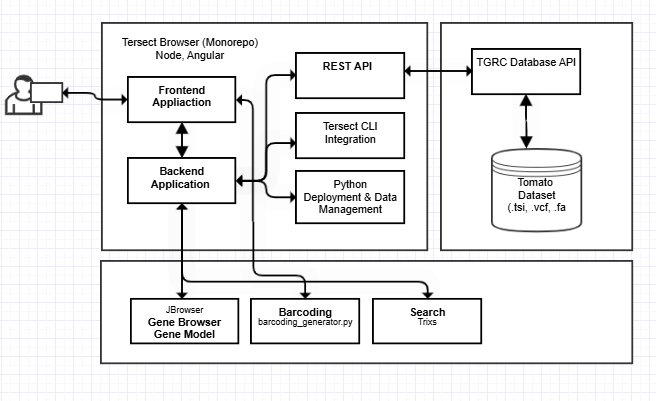
\includegraphics[width=15cm, height=9cm]{high_level_arch_draft.png}
    \caption{Summary Architecture of TersectBrowser+.}
\end{figure}

\subsection{Genome Browser Extension}
\label{sec:Browser}
\subsubsection{Rationale}
The main benefit of TersectBrowser relative to similar genome comparison software for displaying key differences within resequenced datasets is its use of Tersect CLI, to index and then quickly query these genomes for investigation at user-defined scale. However, in order for TersectBrowser+ to be competitive as a tool with other browsers, it was necessary to implement features that enhance further investigation within the scope of the same browser. The main view of the original TersectBrowser displayed the density of variants along each chromosome in comparison to the reference genome. To enhance this view, a variant browser with multiple tracks providing extra information at a per-base level was added to enable to user to directly correlate variant density with accession-specific variants. 

After a review of node-compatible browser tools such as CRAMER, JBrowse was ultimately chosen to carry out this extension request, due to its high customisability, up-to-date features, and active technical support. The initial build of JBrowse into TersectBrowser+ as an extension focused on retaining features most relevant to the user aims, and bringing the styling of the panel in line with the rest of the page. This extension also involved generating a popup window of the same JBrowse component to be initialised when the user was interested in a specific accession or bin region. 

\subsubsection{User Interface}

\paragraph{Feature Description}
\begin{itemize}
    \item JBrowse window:
    \begin{itemize}
        \item Main window is located at the top of Tersect Browser, below settings bar but above the heatmap 
        \item Main window shows only sequence tracks and linear genome scale. Interactive features such as zoom anc chromosome selection have been removed from the main window. The container window has a dynamic offset, which changes according to tree view and zoom level to ensure the chromosome scales between TersectBrowser and JBrowse line up. 
        \item By default, the main window shows only the gene models track.
        \item Popup window provides a more sandbox experience, providing more user interaction. The user can change zoom level and displayed chromosome, and two scale bars enable both precise and rapid navigation. The hamburger menu on the top left provides the capability for the user to upload their own data to visualise unique tracks.
        \item By default, the popup window shows the reference sequence track, gene models track, and variant track for the specified accession.
    \begin{itemize}
        \item \hl{Layout TBC}: Set window size
    \end{itemize}
    \item Tracks:
    \begin{itemize}
        \item Reference sequence 
        \item Variant tracks for each loaded accession
        \item Gene models FeatureTrack (\nameref{sec:Models})
    \end{itemize}
    \item Syncing of the JBrowse window and the TersectBrowser heatmap includes the following:
    \begin{itemize}
        \item Zoom - both by clicking the plus/minus buttons and by scrolling with the mouse wheel.
        \item Bin size.
        \item Selected interval.
        \item Chromosome.
        \item Horizontal scrolling along the x-axis.
    \end{itemize}
\end{itemize}
    
\subsubsection{Technical Description}

\paragraph{View State} 
The \verb +JBrowseLinearGenomeView+ component is imported from @jbrowse/react-linear-genome-view and is wrapped using React. The configurations for the assembly, assembly, and variant tracks, tracks, are imported from the respective assembly.ts and tracks.ts configuration files. The styling configurations, config, are imported from jbrowseConfig.ts. The \verb +JbrowseWrapperProps+ are imported from \verb +JbrowseInterface+. 

The function \verb +JbrowserWrapper+ takes as arguments the props from \verb +JbrowseWrapperProps+ and defines the \verb +viewState+. If an accession has been selected and the accession name is stored under \verb +props.location.accession.name+, the \verb +viewState+ defined in the constant \verb +JbrowseWithAccessionName+ is returned (See below parameters). If not, a conditional check verifies whether the props \verb +defaultInterval+ and \verb +offsetCanvas+ have been populated. If either of them are empty, a container with the phrase "Loading…" is returned. If all data is present, the \verb +viewState+ is defined using the function \verb +createViewState+. This takes as arguments the following variables: 
\begin{itemize}
\item \verb +assembly+: the assembly track 
\item \verb +tracks+: the data tracks to display 
\item \verb +configuration+: the config variable where the theme is defined 
\item \verb +defaultSession+: an object of type LinearGenomeView, which defines the initial state. This object includes the following configurations: 
\begin{itemize}
\item \verb +bpPerPx+: the base pairs per pixel, which defines the bin size 
\item \verb +assemblyName+: the corresponding assembly for the track 
\item \verb +start+: the track start position 
\item \verb +end+: the track end position 
\item \verb +refName+: the genomic coordinates of the viewing window 
\end{itemize}
\end{itemize}

When no accession is selected in the Canvas interface, the first three tracks defined in \verb +tracks.ts+ are added to the \verb +viewState+. The dynamic left-hand offset is set by \verb +horizontalScroll()+. 


\paragraph{Assembly Config}

The configurations for the assembly track, which is built upon the reference accession SL2.50, is defined in \verb +assembly.ts+ in json format. The name is set to the reference accession name and \verb +trackId+ is set to "SL2.50-ReferenceSequenceTrack". The paths to the fasta file, along with its corresponding fasta index, are specified as local server URLs provided by the backend during the Tersect Browser setup. 

\paragraph{Tracks Config} 
The configurations for the \verb +VariantTrack+ and Gene Models \verb +FeatureTrack+ are defined in \verb +tracks.ts+ in json format. For the variant tracks, the \verb +name+ and \verb +trackId+ are set as the accession name, and for the Gene Models track these are set to "ITAG2.4 Gene Models".  The paths to the zipped files, along with its corresponding Tabix index files, are specified as local server URLs provided by the backend during the Tersect Browser setup. Each track is separated by a comma. 

\paragraph{Styling}
The container styling is defined in \verb +jbrowseConfig.ts+. The palette theme is set to colour '\#459e00' and the \verb +boxShadow+ is set to 'none'. 

\paragraph{Zoom} 
The zoom is synchronized between Tersect Browser and the JBrowse component. The \verb +zoomLevel+ observable is a component of the \verb +PlotStateService+ class. Inside \verb +tersect-browser.component.ts+, the subscription \verb +zoomSub+ listens to the \verb +zoomLevel+ observable and assigns the latest value to the component \verb +zoomLevel+. Inside \verb +tersect-browser.component.html+, the \verb +zoomLevel+ is passed to \verb +JbrowseWrapper+ as a prop and is used to define the \verb +bpPerPx+ in the \verb +viewState+. 

The bin size is synchronised in the same way: the \verb +binsize+ observable is a component of the \verb +PlotStateService+ class. Inside \verb +tersect-browser.component.ts+, the subscription \verb +binSizeSub+ listens to the \verb +binsize+ observable and assigns the latest value to the component \verb +binSize+. Inside \verb +tersect-browser.component.html+, the \verb +binSize+ is passed to \verb +JbrowseWrapper+ as a prop. 
Together, \verb +bpPerPx+ is calculated with the following equation: \begin{equation} bpPerPx = ((props.location.binSize) * (100 /props.location.zoomLevel)) \end{equation}


\paragraph{Chromosome selection}
The displayed chromosome is synced in a similar fashion to the zoom and bin size. The \verb +chromosome+ observable is a component of the \verb +PlotStateService+ class. Inside \verb +tersect-browser.component.ts+, the subscription \verb +chromosomeSub+ listens to the \verb +chromosome+ observable and assigns the latest value to the object \verb +selectedChromosomeSub+. Inside \verb +tersect-browser.component.html+, the \verb +selectedChromosomeSub+ is passed to \verb +JbrowseWrapper+ as the prop chromosome. Inside \verb +JbrowseWrapper+, the chromosome name is called from the chromosome object and used to define the \verb +refName+ in the \verb +viewState+. 

Additionally, the default chromosome that is pre-selected when Tersect Browser initially loads is passed to \verb +JbrowseWrapper+ and used to define the default \verb +viewState+. Inside \verb +tersect-browser.component.ts+, the variable \verb +preselectedChromosome+ is defined. On initializing, when the \verb +settings+ observer subscribes to the \verb +tersectBackendService+, the current \verb +plotState.chromosome+ is saved to the \verb +preselectedChromosome+ variable. This is then passed as the prop \verb +preselectedChromosome+ to \verb +JBrowseWrapper+ inside \verb +tersect-browser.component.html+.  Inside \verb +JbrowseWrapper+, the chromosome name is called from the \verb +preselectedChromosome+ object and used to define the \verb +refName+ in the default \verb +viewState+. 


\paragraph{Interval display}
The displayed interval is synced in a similar fashion to the zoom, bin size, and chromosome selection. The \verb +interval+ observable is a component of the \verb +PlotStateService+ class. Inside \verb +tersect-browser.component.ts+, the subscription \verb +selectedIntervalSub+ listens to the \verb +interval+ observable and assigns the latest value to the array \verb +selectedInterval+. Inside \verb +tersect-browser.component.html+, the \verb +selectedInterval+ is passed to \verb +JbrowseWrapper+ as the prop \verb +selectedInterval+. Inside \verb +JbrowseWrapper+, the first element of the array is used to define the start position in the \verb +viewState+, and the second element is used to define the end position. 
Additionally, the default interval that is pre-selected when Tersect Browser initially loads is passed to \verb +JbrowseWrapper+ and used to define the default \verb +viewState+. Inside \verb +tersect-browser.component.ts+, the variable \verb +defaultInterval+ is defined. On initializing, the method \verb +generateMissingSettings+ loads the interval based on the size of the selected chromosome, which is obtained from \verb +BrowserSettings+. The interval is saved as an array to \verb +defaultInterval+ and inside \verb +tersect-browser.component.html+ it is passed as the prop \verb +defaultInterval+ to \verb +JbrowseWrapper+. Inside \verb +JbrowseWrapper+, the first element of the array is used to define the start position in the default \verb +viewState+, and the second element is used to define the end position. 

\paragraph{Offset}
The dynamic offset is synced in a similar fashion to zoom, bin size, chromosome selection, and interval. The observable \verb +offsetCanvas+ is defined as a component of the \verb +PlotStateService+ class. The public variable \verb +offsetCanvasSource+ is defined as an instance of the \verb +BehaviourSubject+ class and holds all recorded values of the canvas offset. In the class constructor, \verb +offsetCanvas+ is initialised to continuously hold the latest value from \verb +offsetCanvasSource+. The canvas offset is set in the \verb +TreePlotComponent+ class, and is passed to \verb +offsetCanvasSource+ when the tree is redrawn. 

Inside \verb +tersect-browser.component.ts+, the variable \verb +offsetCanvas+ is defined, and the subscription \verb +offsetCanvasSub+ listens to the  \verb +offsetCanvas+ observable and assigns the latest value to \verb +offsetCanvas+. Inside \verb +tersect-browser.component.html+, the \verb +offsetCanvas+ is passed to \verb +JbrowseWrapper+ as the prop \verb +offsetCanvas+. Inside \verb +JbrowseWrapper+, the variable defines the extent of the \verb +horizontalScroll+ using the following logic: $horizontalScroll(-(location.offsetCanvas - 4))$. 


\subsubsection{Test Results}
When additional variant tracks are added to the Browser view, the size of the browser panel does not change. The user is able to scroll downwards to view more tracks in the browser. 

When a new dataset is added, the custom addition script automatically updates the names of tracks and assembly in the relevant files within the genome-browser extension. This flexibility allows the Variant Browser extension to be accessible by plant breeders working on many different datasets. TersectBrowser was initially validated with a human genome dataset, so it was important to maintain this flexibility of input in the new extensions.

\subsubsection{Future Improvements}

\subsection{Gene Models Extension}
\label{sec:Models}
\subsubsection{Rationale}
Once the Genome Browser panel was added to the main page of TersectBrowser+, this facilitated the inclusion of a reference gene model track. This allows the plant breeder user to identify an area of high variant density on the heatmap, and then check the gene model track to investigate whether this region occurs near a gene of interest.

\subsubsection{User Interface}
\paragraph{Feature Description}
\begin{itemize}
    \item The gene models track is displayed in the main JBrowse window. 
%    \item Gene model annotations are based on the official \hl{tomato genome annotation v2.4}: \href{https://phytozome-next.jgi.doe.gov/info/Slycopersicum_ITAG2_4#:~:text=Genome%20Overview,genome%2Cwith%2034%2C725%20gene%20models}{Slycopersicum ITAG annotation v2.4}
% The above is tomato-specific. Not sure where it fits. Probably doesn't fit anywhere - included it in notes so that we knew where the tomato gene models came from
    \item In the popup window, the gene models track is displayed as the second track, underneath the reference sequence track and above the variant track.
\end{itemize}

\subsubsection{Technical Description}
The configuration for the Gene Models \verb+FeatureTrack+ is defined as the first entry in \verb+tracks.ts+. The paths to the sorted and compressed GFF file, along with its corresponding Tabix index, are specified as local server URLs provided by the backend during the Tersect Browser setup. 

The Jbrowse \verb+viewState+ is configured in \verb+JbrowseWrapper.tsx+, as described in Extension-JBrowse. If no accession is selected, the first track stored in \verb+tracks.ts+ (gene models track) is added to the \verb+viewState+.

For the popup window, the JBrowse \verb+viewState+ is configured when an accession is selected in \verb+JbrowseWithAccession.tsx+, as described in \nameref{sec:Browser}. If a track with a \verb+trackId+ matching the selected accession is found, the viewer displays the reference sequence track from \verb+assembly.ts+, the first track defined in \verb+tracks.ts+ (gene model track) and the selected accession variant track. 

\subsubsection{Test Results}
This extension has been tested with the additional Soybean dataset, with correct functionality. The relevance of the gene models in the GFF file depend on what the user provides in the dataset, and how the GFF file was created. 

\subsubsection{Future Improvements}

\subsection{Feature Search Extension}
\subsubsection{Rationale}
The aim of this extension is to allow the user to search selected intervals and identify which accessions contain \hl{high/medium/low} impact variants within that region. The bins containing high impact variants for that gene will be highlighted at the accession level, allowing high resolution investigation of variants. The highlighted bins may then be selected and opened in the popup \nameref{sec:Browser} window for further investigation.

\subsubsection{User Interface}
\paragraph{Feature Description}
\begin{itemize}
    \item \verb+Open Variant Search+ button in TersectBrowser+ header, opens popup window for user to select advanced features.
    \item Popup window where user can select interval, choose impact level, and search button to initiate search.
    \item Output: Bins in the canvas are highlighted red at the chromosomal position where the variant is located, and only for accessions containing variants of the specified impact.
    \item Clear button located in TersectBrowser+ header to clear highlighted bins from canvas and restore original heatmmap.
\end{itemize}
\subsubsection{Technical Description}
\paragraph{\hl{Search Bar}}
\paragraph{\hl{Popup window with advanced settings }}
\paragraph{Highlighting bins}
Bin highlighting is controlled in the \verb+bin-draw.service+ by two functions. The first function, \verb+highlightFeatureBins()+, is defined, taking as arguments a string containing accession names, the bin position along the x-axis, and the \verb+binView+. First, the y-axis bin position for accession names is calculated. Then, the \verb+binView+ is redrawn in greyscale, with the bin colour determined by the difference to the reference accession. Using the x-axis \verb+binIndex+ position and the y-axis accession bin positions, these bins are coloured red in the \verb+binView+. The modified \verb+binView+ is returned as the output. The second function, \verb+highlightBins()+, takes as arguments the start position of the interval and the bin size currently shown in the Tersect pane, a list of ordered accessions shown in the canvas, and the searched accessions. For each searched accession, accession name is reformatted to match the format displayed in the Tersect pane. Then, the bin position along the x-axis is calculated using the \verb+getBinIndexFromPosition()+ function, which takes as arguments the feature position along the chromosome, the interval start position, and the bin size. Then, \verb+highlightFeatureBins()+ is called for each accession. Lastly, the canvas is redrawn using the modified \verb+binView+ output from \verb+highlightFeatureBins()+. 
\begin{itemize}
    \item highlightFeatureBins(accessions: string[], binIndex: number, binView: DistanceBinView) - takes a string of accession names, a binIndex (corresponding to the bin position along the x-axis matching the gene position on the chromosome), and binView. The y-axis index for bins matching accession names in the accessions strings is calculated and combined with the binIndex to colour these specific bins red. The rest of the bins are coloured in greyscale, with saturation depending on binDistance (calculated from tersect on the backend 
    \begin{itemize}
        \item Bin-draw.service.ts 
        \item Called by highlightBins() in bin-draw.service.ts 
    \end{itemize}
    \item highlightBins(intervalStart, binsize, orderedAccessions, searchedAccessions) - takes selected interval start position, selected binSize, list of ordered accessions shown in the canvas, and searched accessions (passed from callback function?). Accession names in Jbrowse are in a different format to what is stored in tersect browser, so accession names are reformatted to match tersect browser bins. binIndex is calculated for the selected gene. These two are passed to highlightFeatureBins() - along with this.bins - to highlight the bins. The canvas is then redrawn using the binView calculated in highlightFeatureBins(). 
    \begin{itemize}
        \item Bin-draw.service.ts 
        \item Called by callHighlightBins() in tersect-browser.component.ts 
    \end{itemize}
    \item callHighlightBins(searchedAcessions) - takes searchedAccessions. Calls highlightBins(), passing along  selected interval start position, selected binSize, list of ordered accessions shown in the canvas, and searched accessions (passed from callback function?). 
    \begin{itemize}
        \item Tersect-browser.component.ts 
    \end{itemize}
\end{itemize}

\paragraph{Calling Highlighting Bins} \mbox{}
\\
\hl{TBC: Mechanism} of searching VCFs to identify variants 

Finally, callHighlightBins() is called, which itself calls highlightBins() from the bin-draw.service, passing as arguments the current interval start position, binsize, displayed accessions in an ordered format, and the searched accessions.  
\paragraph{\hl{Clear Button }}
The clear button is located to the right of the \verb+Open variant search+ button and styled with \verb+fa fa-refresh+. It contains the event handler \verb+(click)="refreshBin()"+ that calls the \verb+refreshBin()+ method in \verb+BinDrawService+.
This method calls \verb+generatePlotArray()+, which re-creates the bin view, and \verb+updateCanvas()+, which redraws the canvas using the re-created bin view.
 

\subsubsection{Test Results}
\subsubsection{Future Improvements}


\subsection{Barcode Generation Extension}
\subsubsection{Rationale}
A key aim for plant breeders when comparing their own plant strains with other cultivars in resequenced datasets is to be able to identify their strain at the genome level. 
This would allow for protection of intellectual property in the case of an advantageous new introgression that can be uniquely identified. 
The Barcoding extension allows this unique accession-specific identification by generating a range of barcodes with a user-specified length and maximum number of SNPs,
so that the barcodes are easily analysed in wetlab environments. Metrics comparing these putative barcodes are also provided to the user, and available for local download. 

\subsubsection{User Interface}

\begin{figure}[h]
    \centering
    \includegraphics[width=5cm, height=9cm]{UserBarcode.jpg}
    \caption{User-focused data flow through Barcoding Extension.}
\end{figure}
\paragraph{Frontend Display Feature Description}
When the user clicks on a bin, the popup menu appears and the button "Create barcode" is visible, styled with a barcode icon. When the user clicks on this button, a popup window appears in the centre of the screen. The window title is the corresponding accession name. The window contains the header "Barcode Generator" and contains a description of what is being generated. There is a box for the user to input barcode size, with default set to 150, and the maximum number of variants allowed per barcode (this is an optional parameter. Leaving this blank means all possible barcodes will be returned).  

At the bottom is a green "Generate" button. Hovering over the button turns it dark green, and clicking on this button will call the backend scripts to generate the barcodes output. Whilst scripts are running and barcodes are being generated, a spinner is added to the button to indicate loading. After the script has been generated, the spinner disappears and another green button "Download" appears at the bottom left of the window. Clicking on the button downloads the tsv file containing the barcodes.  

\paragraph{Backend Script Feature Description}
Given input parameters specified by the user, barcodes are generated via the backend and can be downloaded in tsv format. The downloaded file is titled in the following format for easy identification and to prevent files being overwritten: \textit{SystemDateAndTime\_TB\_Barcode\_Gen\_AccessionName\.txt}.

The file contains the following information: 
\begin{itemize}
    \item \textbf{Barcode sequence} - The base with the accession-specific SNP is enclosed in square brackets.
    \item \textbf{Chromosome} - The chromosome on which the barcode is located.
    \item \textbf{Barcode Start \& Barcode End} - The absolute position of the barcode in the chromosome.
    \item \textbf{Variant Count} - The number of accession-specific SNPs that are present in the barcode.
    \item \textbf{Variant Position} - The relative position of the accession-specific SNPs in the barcode. 
    \item \textbf{Repeat Sequence} - The sequence of the 2-bp repeating region. A repeating region is defined as 2 base pairs repeating 3+ times. 
    \item \textbf{Repeat Multiplier} - The number of times the repeat sequence is repeated.
    \item \textbf{Repeat Start-End} - the relative start and end position of the repeat region within the barcode sequence. 
    \item \textbf{GC Content} - The GC content of the barcode. 
\end{itemize}


\subsubsection{Technical Description}


\begin{figure}[h]
    \centering
    \includegraphics[width=7cm, height=12cm]{ExtBarcode.jpg}
    \caption{User-focused data flow through Barcoding Extension.}
\end{figure}

Barcode generation is controlled by two scripts: \verb+barcode_finder.sh+ and \verb+find_barcode.py+. 

\paragraph{Bin menu barcode button}:\\
A third menu item with the label \verb+Create barcode+ is added to the \verb+getAccessionItem()+ method in \verb+plot-click-menu.component+. The item is styled with the \verb+fa fa-barcode+ icon, and on command opens the \verb+ModalService openBarcodeModal()+ method, passing as arguments the plot state chromosome name and the bin accession label and start and end positions.

\paragraph{Modal Service Component}:\\
The observables \verb+barcodeVisible$+, \verb+barcodeTitle$+, \verb+barcodeChromo$+, \verb+barcodeStart$+ and \verb+barcodeEnd$+ are added to \verb+modal.service+. The method \verb+openBarcodeModal()+ is added, accepting as arguments \verb+accessionName+, \verb+chrom+, \verb+startPosition+, and \verb+endPosition+. These arguments are saved to their corresponding observables.  

A new modal, \verb+global-barcode-modal+, is created. The modal is imported to app.module and added to app.component. The \verb+global-barcode.component.ts+ imports \verb+ModalService+ and \verb+TersectBackendService+. Variables to hold the modal state, modal loading state, modal title, barcode size, chromosome, interval start position, interval end position, maximum variants per barcode, the downloadable URL and filename are defined. On initialisation, modal state, modal title, chromosome, interval start position and interval end position are saved to observables in modal.service. 

The method \verb+generateBarcode()+ calls and subscribes to the \verb+tersectBackendService generateBarcodes()+ method, setting the \verb+isLoading+ constant to "True" and passing as arguments \verb+modalTitle+, \verb+chromosome+, \verb+startPosition+, \verb+endPosition+, \verb+barcodeSize+, and \verb+maxVariants+. The returned URL and filename are saved to the variables \verb+downloadUrl+ and \verb+downloadFileName+. Once returned, \verb+isLoading+ is set to "False" and \verb+barcodeSize+ is set back to "150". 

The popup window is reset when closed by \verb+resetModal()+ on closing, which sets the \verb+barcodeSize+ to "150", \verb+maxVariants+ and \verb+downloadUrl+ to null, and \verb+downloadFileName+ to an empty string, removing the "Download" button from the popup.  

\paragraph{Modal Service Styling}:\\
The modal template is defined in \verb+global-barcode.component.html+. The popup window is visible depending on the modal state isVisible, and is centrally position with \verb+modalTitle+ set as the header. Explanation about the barcode service is described in the \verb+modal-title+ and \verb+modal-subtitle+ divs, and the \verb+input-container+ div contains input boxes for barcode size and maximum number of variants, the button "Generate" which calls \verb+generateBarcode()+ and simultaneously shows a \verb+progressSpinner+ whilst the barcodes are being generated. An anchor displays a clickable "Download" p-button that points towards the generated barcode file. The filename is set to \verb+downloadFileName+, and "Download" is only visible once a \verb+downloadUrl+ has been generated for the barcodes file.  

Styling is defined in the \verb+global-barcode.component.css+. Button background colour is set to \verb+#459e00+, background hover colour is set to \verb+#33b357+, and text colour is set to white. The input boxes and labels are given a set width of 200px. 

\paragraph{Router and Backend service}:\\
A new route, \verb+/generate-barcodes+, is added to \verb+tersect-router+. This router receives in the request the following parameters: \verb+accessionName+, \verb+chrom+, \verb+start+, \verb+end+, \verb+size+ and \verb+maxVar+. Paths to the tsi index and fasta file are defined. The backend script, \verb+barcode_finder.sh+, is called, with the above parameters passed as arguments. A \verb+downloadableURL+ is created, pointing to the created file, and returned in json format.  

The method \verb+generateBarcodes()+, is added to \verb+tersect-backend.service+. It sends a HTTP Post request to the endpoint \verb+/generate-barcodes+, triggering barcode generation. The method returns an observable containing the \verb+downloadableURL+ pointing to the generated barcode file. The method passes the following parameters: 
\begin{itemize}
    \item \textbf{accessionName} - a string containing the specified accession name for which to generate unique barcodes 
    \item \textbf{Chrom} - a string containing the chromosome identifier for the chromosome where the barcodes will be generated 
    \item \textbf{Start} - a number specifying the start position of the interval in which to generate barcodes 
    \item \textbf{End} - a number specifying the end position of the interval in which to generate barcodes 
    \item \textbf{Size} - a number specifying the length of the barcodes 
    \item \textbf{maxVar} - an optional parameter, specifying the maximum permissible number of variants located within the barcode. Either a number or null, indicating all barcodes with all numbers of variants are generated
\end{itemize}


\paragraph{Calling Tersect CLI to extract variants}: \\
\verb+Barcode_finder.sh+ is run on the command line, and takes as input accession name, chromosome, interval start position, interval end position, barcode size, maximum variant number, reference fasta, and tersect TSI index. The chromosome and interval start and end positions are used to define the searchable \verb+REGION+, and the accession name is used to define \verb+SAFE_ACC+ which is used to save files to a temporary file.  

The tersect CLI command \verb+tersect view+  is called to extract all variants within the specified region for the specified accession. The output is saved as a temporary TSV file as: \verb+${SAFE_ACC}_acc_unique.tsv+. The tersect CLI command tersect view is again used to extract all variants within the specified region for all accessions except the specified accession. This output is saved as a temporary TSV file as: \verb+${SAFE_ACC}_union_vars.tsv+.  

Lastly, the \verb+find_barcode.py+ file is called, passing as arguments the accession name, reference fasta, chromosome, interval start position, interval end position, barcode size, maximum variant number, and the tersect output files  \verb+${SAFE_ACC}_acc_unique.tsv+ and  \verb+${SAFE_ACC}_union_vars.tsv+. 

\paragraph{Generating barcodes}: \\
\verb+Find_barcode.py+ requires the following dependencies: argparse, SeqIO, and datetime.  

The reference fasta is parsed using \verb+SeqIO.parse+, yielding sequence records that are converted to a dictionary using \verb+SeqIO.dict+. Using the user-inputted chromosome name, \verb+[args.chrom].seq+ extracts the chromosome sequence from the dictionary and saves it to the variable ref. The user-defined interval start and end positions are used to extract the \verb+ref_window+ from ref. 

The \verb+load_variant_file()+ method imports the tersect output files and creates a dictionary, with variant position being stored as the key and a tuple containing the original base and the alternate base being stored as the dictionary value. Then, the \verb+remove_overlapping_variants()+ method compares the dictionaries and creates a new dictionary \verb+new_unique_vars+ with the same format, containing variants that are only present in the specified accession and not also present in any other accession. The method \verb+apply_variants_to_sequence()+ then uses the \verb+ref_window+ and \verb+new_unique_vars+ to generate an accession-specific sequence, \verb+unique_seq+, containing accession-specific SNPs. Lastly, the \verb+find_barcode_windows()+ method compares \verb+unique_seq+ against \verb+ref_window+ and using a sliding window of 1 base pair, identifies regions where the two sequences differ. The sequence, along with the absolute start and end position, is saved to the variable barcodes.  

\paragraph{Output file and barcode stats}: \\
Statistical metrics are calculated for each barcode, using custom methods. The number of accession-specific variants is calculated using \verb+count_variant_number()+, which also records variant position within the barcode. The variant position is used to highlight the variants within the barcode using the custom \verb+highlight_ref_alt_positions()+ method, which encloses the variant in the following format: \verb+[original base/alternate base]+. Repeat content is calculated using \verb+find_dinucleotide_repeats_custom()+, with repeats being defined as regions where a dinucleotide (2-base pair) sequence repeats consecutively three or more times. The repeating dinucleotide, number of times the dinucleotide repeats, and the start and end positions of the repeat region within the barcode are returned. GC content is calculated as a percentage to six decimal places using \verb+calculate_gc_content()+. 

The barcodes and respective metrics are written to a tsv file. The file name is formatted to include system date and time, \verb+'TB_Barcode_Gen'+, and the specified accession. 

\subsubsection{Test Results}
\subsubsection{Future Improvements}
\subsection{Future Work and Extension Design}
\subsubsection{Automated Introgression Search Extension}

\section{APPENDICES}

\section {References}


\end{document}
